\section{Results}
\label{sec:experiments}


We analyze $121$ evolutionary runs across the four frameworks of Table~\ref{tab:frameworks}, $16$ tasks spanning Python mathematical constructions and C++ ALE-bench problems (\texttt{ahc008}--\texttt{ahc046}), and $5$ LLMs varied with and without diff-based generation (whether the LLM emits a unified diff or a full rewritten program). Each run consists of $100$ search iterations. Aggregate program-, call-, and token-level statistics are reported in Appendix~\ref{appendix:experiment-scale}.

\subsection{Static analysis: what gets evolved?}
\label{sec:static-analysis}

We characterize the typical behaviour of evolutionary coding frameworks across our $121$ runs. Programs do change shape during search (Figure~\ref{fig:loc-hparam}): math runs accumulate modest LOC and numeric-literal growth, while ALE runs are refined at near-constant size from already-large seeds. The figure serves as backdrop for the math-comparison difficulty discussed next and for the BO-ceiling probe of \S\ref{sec:tuning-gap}; the more interesting question is what these changes contribute, which we address through edit-level analysis below.

\begin{figure}[t]
\centering
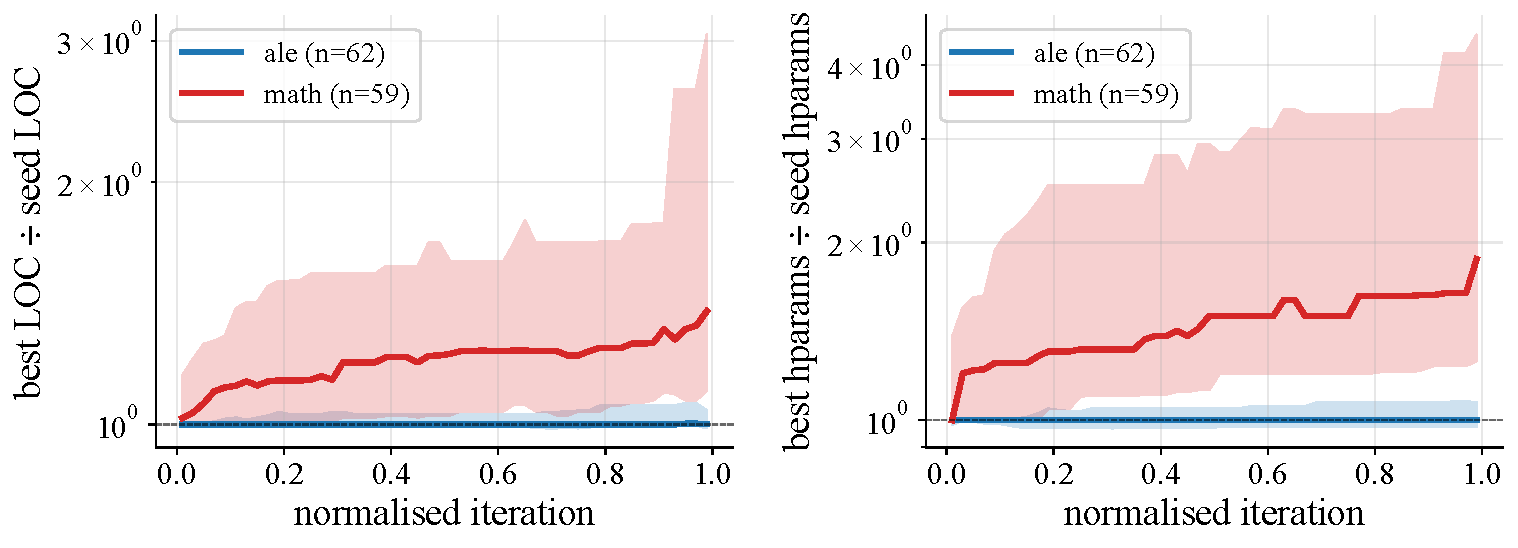
\includegraphics[width=0.95\linewidth]{static_analysis/figures/F1_loc_hparam.pdf}
\caption{\textbf{Program size and numeric-literal hyperparameter count over a run.} Best-so-far program length (LOC, left) and numeric-literal count (right), each normalized by the run's seed value, plotted against normalized iteration. Solid line = cross-run median; shaded band = inter-quartile range; dashed gray line marks the seed value. Math runs ($n{=}59$) accumulate modest LOC and hp growth (median final ratios $1.33\times$ and $1.70\times$); ALE runs ($n{=}62$) refine large seeds in place (final ratio $\approx 1.0\times$ on both axes).}
\label{fig:loc-hparam}
\end{figure}

\paragraph{Lineage depth and budget utilization.}
The chain of parents from each final-best program back to the seed is short in both domains, but is somewhat shorter on ALE (median lineage depth $4$, vs.\ $6$ on math). On math the median best-so-far is reached around iteration $0.75$ of the budget, while on ALE it lands earlier (median normalized iteration $0.49$). In both cases the dominant pattern is jackpot-then-flat: most of the per-run iteration budget is spent on dead branches that do not contribute to the final best.

\paragraph{Public-vs-private generalization on ALE.}
ALE-bench public scores are not the held-out judging metric. Re-scoring every ALE run's public best-so-far chain on the private test set used by AtCoder ($n{=}30$ run/problem pairs across the four main backends), two of the four frameworks overfit on at least $30\%$ of the problems they were scored on, and the same problem can flip generalization sign across frameworks: on \texttt{ahc024}, OpenEvolve found a $+1{,}606$ rating-point private gain while ShinkaEvolve, on the same problem, \emph{lost} $1{,}610$ rating points despite a positive public score change. The public best-so-far chain is therefore unreliable as a single-number summary on ALE; full per-problem and per-framework tables are in Appendix~\ref{appendix:public-private}.

\paragraph{Edit taxonomy via LLM-as-judge.}
We use EvoReplay's LLM-as-judge pipeline (\S\ref{sec:evoreplay}, capability (b)) to annotate every parent--child edit with one or more categories from a 9-label taxonomy (\emph{Hyperparameter tuning}, \emph{Local refinement}, \emph{Architectural change}, \emph{Composition}, \emph{Efficiency}, \emph{Bug fix}, \emph{External dependency}, \emph{Pruning}, and \emph{Refactor}, applied to every parent--child edit in EvoTrace across the four backends. Agreement between the judge and a blind human re-annotation on a stratified sample of $200$ edits is substantial overall (macro $\kappa = 0.77$, micro-$F_1 = 0.90$, exact-match accuracy $74.5\%$), with per-category breakdowns and the one failure case (\emph{external\_dependency}) reported in Appendix~\ref{appendix:judge-validation}. The picture splits cleanly into a frequency view and a per-edit utility view (Figure~\ref{fig:edit-taxonomy-results}).
By frequency, \emph{Hyperparameter tuning} is the single most prevalent label, consistent with the cycling pattern of \S\ref{sec:cycling} and the tuning-gap analysis of \S\ref{sec:tuning-gap}. By per-edit utility, however, the strongest categories are different: \emph{External dependency} edits have a $3.58\times$ odds ratio for positive normalized score change ($n{=}104$), \emph{Efficiency} $1.61\times$ ($n{=}464$), and \emph{Architectural change} $1.55\times$ ($n{=}1{,}075$).
The frequency--utility gap propagates to successful trajectories: best-so-far updates and final-best lineages are both enriched in \emph{Efficiency}, \emph{External dependency}, and \emph{Hyperparameter tuning} relative to the all-edits base rate (Appendix~\ref{appendix:edit-taxonomy-aggregate}). Edits are typically multi-label ($67.4\%$ have $\geq 2$ labels), so these categories should not be read as mutually exclusive modes; the most common compound patterns are \emph{Hyperparameter tuning + Local refinement} and \emph{Composition + Hyperparameter tuning}.

\begin{figure}[t]
\centering
\begin{minipage}[b]{0.49\linewidth}
  \centering
  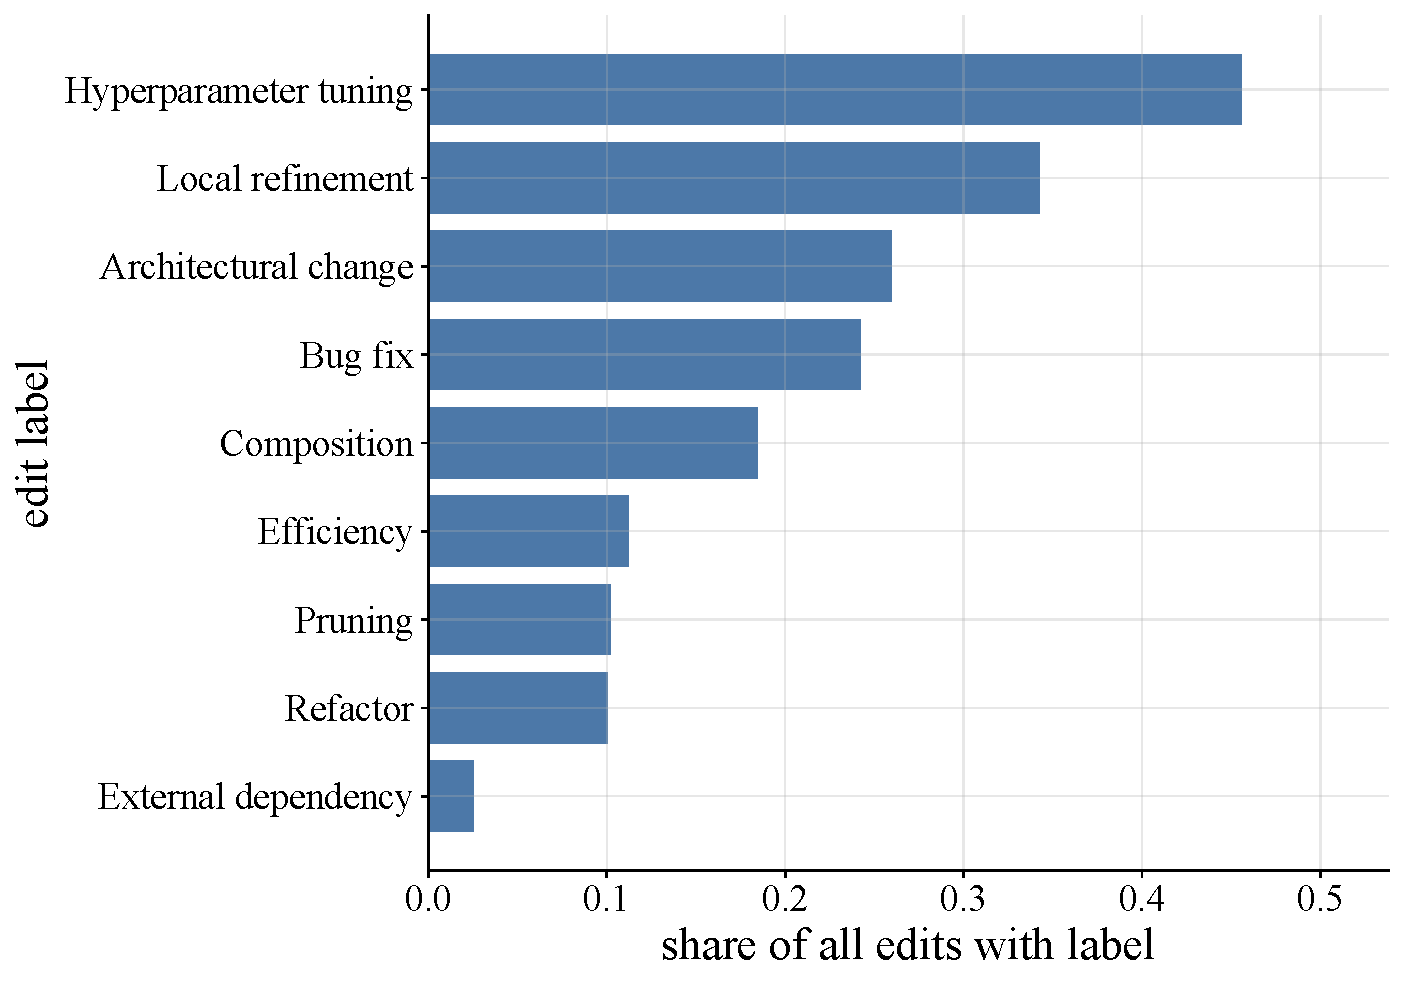
\includegraphics[width=\linewidth]{paper_package_edits/main_figures/edit_label_prevalence.pdf}\\
  {\small (a) Prevalence}
\end{minipage}\hfill
\begin{minipage}[b]{0.49\linewidth}
  \centering
  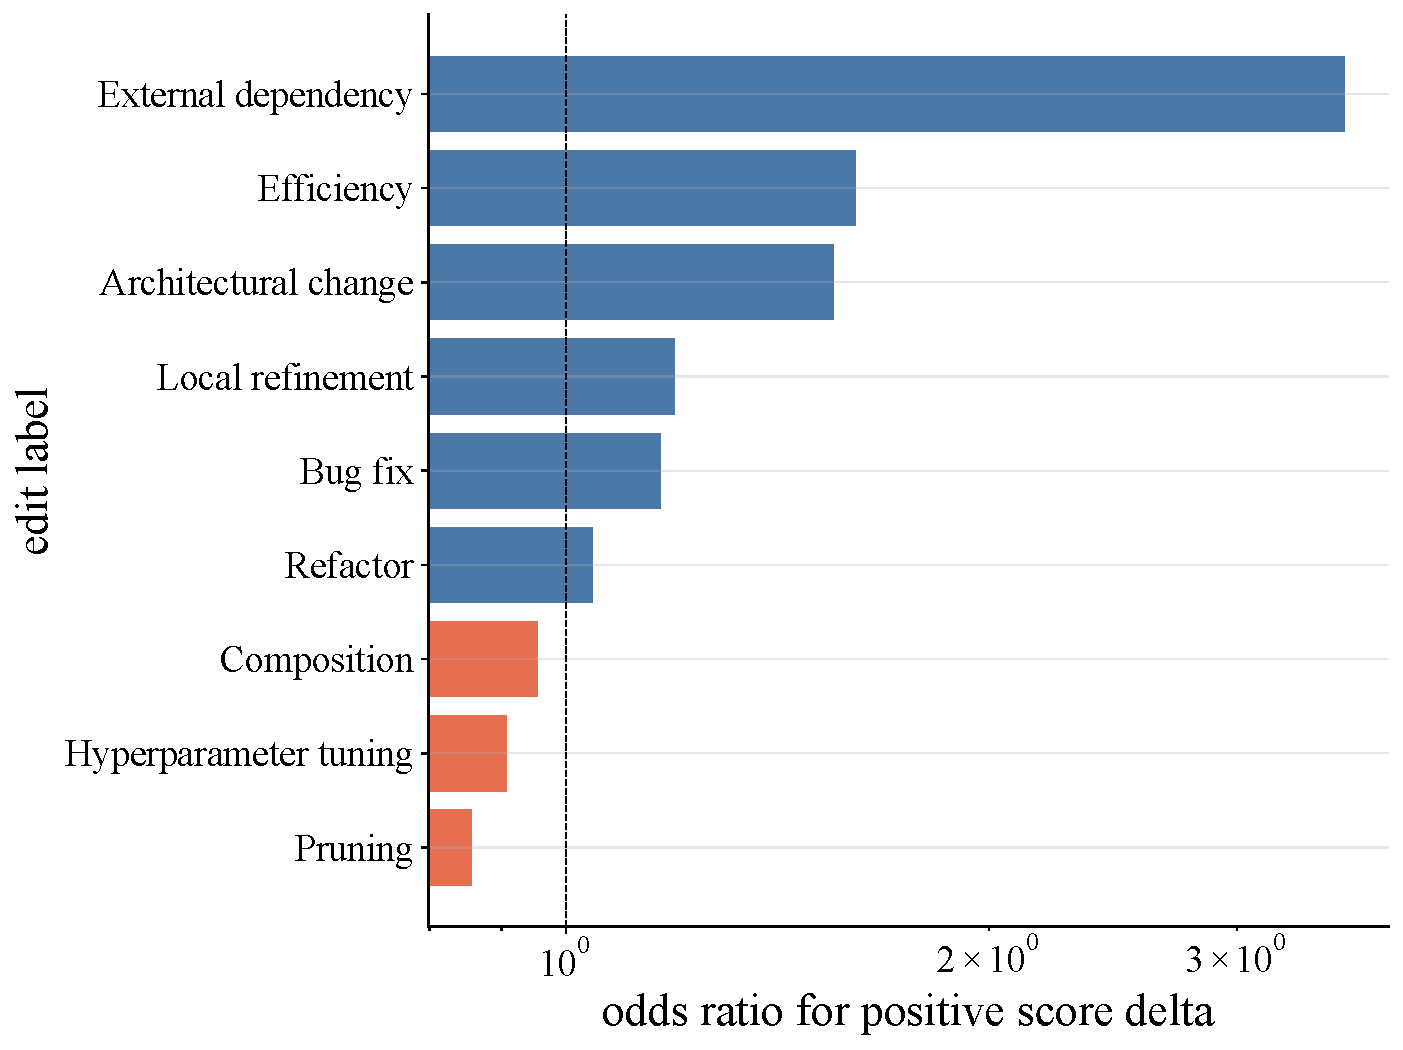
\includegraphics[width=\linewidth]{paper_package_edits/main_figures/edit_helpfulness_odds_ratio.pdf}\\
  {\small (b) Helpfulness (odds ratio)}
\end{minipage}
\caption{\textbf{Edit-taxonomy: frequency vs.\ per-edit utility} across all programs in EvoTrace. \textbf{(a)}~Frequency of each label: \emph{Hyperparameter tuning} dominates the search distribution. \textbf{(b)}~Per-edit odds ratio for positive normalized score change: \emph{External dependency}, \emph{Efficiency}, and \emph{Architectural change} are the most helpful categories on a per-edit basis. The categories that most often improve a single edit are not the categories the search spends most of its effort on. Best-so-far and final-best-lineage enrichment views, plus per-domain and per-backend breakdowns, are in Appendix~\ref{appendix:edit-taxonomy-aggregate} and Appendix~\ref{appendix:edit-taxonomy-breakdowns}.}
\label{fig:edit-taxonomy-results}
\end{figure}

\finding{The categories that most often improve a single edit (\emph{External dependency}, \emph{Efficiency}, \emph{Architectural change}) are not the categories evolutionary search spends most of its effort on (\emph{Hyperparameter tuning}, \emph{Local refinement}). Most score gains come from a small subset of edit types, and that subset is rare in the search distribution.}

\subsection{Cycling: re-introducing previously deleted code}
\label{sec:cycling}

While manually inspecting traces to derive the edit taxonomy, we repeatedly observed lineages re-introducing lines they had earlier deleted, so we operationalized this as a deterministic check: for each parent--child diff, how often is an \emph{added} line byte-identical to a line that the same lineage has already \emph{deleted} in an earlier iteration? Across all $121$ runs, the median share of added lines that are such re-introductions is $\sim\!30\%$, and this rate grows monotonically over the run in $118$ of $121$ cases (median per-iteration slope $+0.0030$). Cycling is present throughout the trajectory of essentially every run we measure, not a late-run pathology, and is dominated by short-span churn (median $5$ iterations between deletion and re-introduction); the signal is stable across all four frameworks, both languages, and all $5$ generator models we tested. A walk-through of one short-span cycle is given in Appendix~\ref{appendix:cycling-example}, with additional analyses (a finer three-way recycling classifier, a model- and prompt-dependence breakdown, and a null result on post-breakthrough cycling) in Appendix~\ref{appendix:cycling-extras}.

\finding{Roughly $30\%$ of code lines added during evolutionary search are byte-identical to lines previously deleted in the same lineage, and the cycling rate grows monotonically over the run in $118$ of $121$ cases. Search budget is partly spent re-introducing material the run has already discarded, a deterministic and reproducible signal that is present throughout each run and across all frameworks, languages, and generator models we tested.}

\subsection{Replay reproducibility: structural, not lexical}
\label{sec:replay}

When evolutionary search reaches a new best-so-far program, can we reproduce that breakthrough by re-running the same prompt? For each of $36$ best-so-far events across the four backends, we re-prompted an LLM $10$ times with the exact context the original run had used and asked four questions of each replayed program: does it run? does the evaluator accept it? does it match the original program byte-for-byte? does it match the original score? Table~\ref{tab:replay-summary} reports the medians and four illustrative targets covering the recurring patterns.

\finding{Replays almost always produce a runnable program (median parse and evaluator success $1.00$) but essentially never the original program (median exact-match $0.00$). They nevertheless recover a median $0.76$ of the original score from a \emph{different} program: the score gain is broadly reproducible from the same prompt context even though the specific program is not.}

\begin{table}[t]
\centering
\caption{\textbf{Replay summary across $36$ breakthrough events.} Aggregate medians and four illustrative targets covering recurring replay patterns. ``Replay/Original'' is the median replayed score divided by the original program's score.}
\label{tab:replay-summary}
\small
\setlength{\tabcolsep}{4pt}
\renewcommand{\arraystretch}{1.15}
\begin{tabular}{@{}lccccl@{}}
\toprule
Target & Parse & Eval & Exact & Replay/Orig.\ & Pattern \\
\midrule
\textbf{Median across $36$ targets} & $1.00$ & $1.00$ & $0.00$ & $0.76$ & --- \\
\midrule
\texttt{circle\_packing\_iter68\_improve}    & $1.00$ & $1.00$ & $\geq\!0$ & $\approx\!1.00$ & tight reproduction \\
\texttt{second\_autocorr\_iter79\_improve}   & $1.00$ & $1.00$ & $0.00$    & $0.96$          & parent-revert \\
\texttt{circle\_packing\_iter32\_neutral}    & $0.50$ & $0.50$ & $0.00$    & ---             & bimodal failure \\
\texttt{heilbronn\_convex\_iter100\_regress} & $1.00$ & $1.00$ & $0.00$    & $1.11$          & replays exceed regress.\ \\
\bottomrule
\end{tabular}
\end{table}

\subsection{The tuning gap: how much is just hyperparameter search?}
\label{sec:tuning-gap}

\newcommand{\NBOwins}{22}
\newcommand{\NBOnochange}{8}
\newcommand{\NBOregress}{6}

We separate a program $p$ into a structure $s$ and a hyperparameter vector $\theta \in \Theta_s$ it exposes, writing $p = s(\theta)$. Holding $s_0$ fixed and running Bayesian optimization over $\theta$ yields a tuning ceiling $f^{\star}_{\mathrm{BO}}(s_0) = \max_{\theta} f(s_0(\theta))$, and the \emph{tuning gap} $\Delta(s_0) = f^{\star}_{\mathrm{evo}} - f^{\star}_{\mathrm{BO}}(s_0)$ measures how much of the evolutionary gain reflects structural discovery rather than parametric search. We operationalize $f^{\star}_{\mathrm{BO}}$ with one \texttt{deepseek-reasoner} call that proposes per-knob log/linear intervals, an automatic rewrite to a top-level \texttt{PARAMS} block, and a $24$-call \texttt{gp\_minimize} ($8$ random $+ 16$ BO acquisitions; full pipeline in Appendix~\ref{appendix:bo-details}).

\begin{wraptable}{r}{0.42\textwidth}
\vspace{-1.0em}
\centering
\caption{BO outcomes on $36$ mid-run programs (median $6$ knobs per program; $24$ evaluator calls each).}
\label{tab:bo-outcome}
\small
\setlength{\tabcolsep}{8pt}
\renewcommand{\arraystretch}{1.15}
\begin{tabular}{@{}lr@{}}
\toprule
\textbf{Outcome} & \textbf{\# targets} \\
\midrule
BO improves over original & \NBOwins{} \\
No change                 & \NBOnochange{} \\
BO regresses              & \NBOregress{} \\
\midrule
\textbf{Total}            & \textbf{36} \\
\bottomrule
\end{tabular}
\vspace{-0.6em}
\end{wraptable}

\paragraph{BO matches the evolutionary run's final-best on most intermediate programs.}
On $36$ intermediate programs sampled across runs, frameworks, and models, BO improves over the program's original score in \NBOwins{} of $36$ cases (Table~\ref{tab:bo-outcome}). When compared against the run's \emph{final}-best score (rather than the program's original score), BO matches or exceeds it on $13$ of $15$ intermediate programs (median delta $+0.025$). The largest individual gain is on \texttt{heilbronn\_tri\_dsr\_nodiff}, where the evo run reached $0.521$ in $100$ iterations and BO on an intermediate program from the same run reached $0.886$ ($1.70\times$ the evo final-best). The strong dependence of $f^{\star}_{\mathrm{BO}}(s_0)$ on $s_0$'s exposed knobs complicates math-benchmark cross-framework comparison: two frameworks with similar topology but different knob exposures give different headline scores even with identical search behaviour, so the defensible per-target summary is the pair $\big(f(p_0),\, f^{\star}_{\mathrm{BO}}(s_0)\big)$.

\finding{A $24$-call Bayesian-optimization pass on a single intermediate program's exposed hyperparameters improves over the program's score in \NBOwins{} of $36$ probed targets, and matches or exceeds the evolutionary run's final-best score on $13$ of $15$ intermediate programs (median delta $+0.025$). On these targets, late evolutionary iterations on math are largely matched by post-hoc hyperparameter tuning of an earlier program.}

